
\begin{tikzpicture}
\begin{axis}[
width=1.00\textwidth,
height=6cm,
name=forcedImp15,
ylabel=${u_{x,y}\,\mathrm{[L\,T^{-1}]}}$,
xlabel=${t\,\mathrm{[T]}}$,
xmin = 0.0,
xmax = 2.0,
ymin = -0.02,
ymax = 0.10,
y tick label style={
                /pgf/number format/.cd,
                fixed,
                fixed zerofill,
                precision=2,
                /tikz/.cd
            },
legend style ={
                at={(1.1 ,0.5)}, 
                anchor=east, %north west
                draw=black, 
                fill=white,
                align=left,
                legend columns=1,
            },
]
\addplot+ [mark=none,black,style=solid,thick]table [x={t}, y={Ux1}] {\myGraphs/forcedImpeller/URED_11_RE15_CFD};
\label{Ux}
\addplot+ [mark=none,black,style=solid,thick,dashed,thick] table [x={t}, y={Uy1}] {\myGraphs/forcedImpeller/URED_11_RE15_CFD};
\label{Uy}
\addplot+ [mark=none,blue,style=solid,thick]table [x={t}, y={Ux1}] {\myGraphs/forcedImpeller/URED_11_RE15_hex_V18-V9-IsozIVOF6};
\label{hex}
\addplot+ [mark=none,blue,style=solid,thick,dashed] table [x={t}, y={Uy1}] {\myGraphs/forcedImpeller/URED_11_RE15_hex_V18-V9-IsozIVOF6};
\addplot+ [mark=none,orange,style=solid,thick]table [x={t}, y={Ux1}] {\myGraphs/forcedImpeller/URED_11_RE15_tri_V18-V9-IsozIVOF6};
\label{tri}
\addplot+ [mark=none,orange,style=solid,thick,dashed] table [x={t}, y={Uy1}] {\myGraphs/forcedImpeller/URED_11_RE15_tri_V18-V9-IsozIVOF6};
\addplot+ [mark=none,green,style=solid,thick]table [x={t}, y={Ux1}] {\myGraphs/forcedImpeller/URED_11_RE15_poly_V18-V9-IsozIVOF6};
\label{poly}
\addplot+ [mark=none,green,style=solid,thick,dashed]table [x={t}, y={Uy1}] {\myGraphs/forcedImpeller/URED_11_RE15_poly_V18-V9-IsozIVOF6};



\node [draw,fill=white,anchor=south] at (rel axis cs: 0.5,0.3) {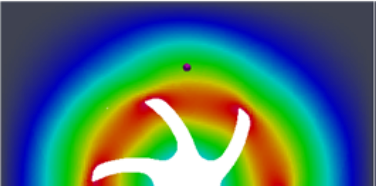
\includegraphics[width=0.35\textwidth]{\myGraphs/forcedImpeller/probePlacementV0.png}};
\draw[color=white,fill=white] (rel axis cs: 0.30,0.57) rectangle (rel axis cs: 0.4,0.8);
\draw[->, thick,font=\small] (rel axis cs: 0.31,0.6)--(rel axis cs: 0.36,0.6) node[right]{$x$};
\draw[->, thick,font=\small] (rel axis cs: 0.31,0.6)--(rel axis cs: 0.31,0.75) node[right]{$y$};

\node [draw,fill=white,anchor=north west,font=\small] at (rel axis cs: 0.1,0.75) {\shortstack[l]
{
\ref{Ux} $u_{x}$ \\
\ref{Uy} $u_{y}$ }};
\node [draw,fill=white,anchor=east,font=\small] at (rel axis cs: 0.99 ,0.5) {\shortstack[l]
{
\ref{Ux} CFD\\
\ref{hex} hexMesh\\
\ref{tri} triMesh\\
\ref{poly} polyMesh
}};

\end{axis}
\node[left=1.0cm,anchor=east] at (forcedImp15.north west) {(a)};
\end{tikzpicture}
